\documentclass[11pt,a4paper,final]{report}
\usepackage[utf8]{inputenc}
\usepackage[norsk]{babel}
\usepackage{amsmath}
\usepackage{amsfonts}
\usepackage{amssymb}
\usepackage{graphicx}
\usepackage{verbatim}
\usepackage[left=2cm,right=2cm,top=2cm,bottom=2cm]{geometry}
\author{Krister Borge \\Hamza Muftic \\Barthas Venkcus}
\title{Oblig 2 }
\begin{document}
\maketitle


Placement of images is hard in latex, therefor the images is on the last page.
\section{ Task1 }

	Both a $Vds > vt$ for strong inversion and a $ Vds<vt$ for weak inversion.
\begin{figure}[h!btp]
\caption{Task 1}
\includegraphics[scale=1]{1task1.png}
\end{figure}

	logaritmic scale
	
\begin{figure}[h!btp]
\caption{Task 1 logaritmic}
\includegraphics[scale=1]{1task1log.png}
\end{figure}


\begin{verbatim}
Vgs=linspace(0, 5, 51)';
sIds=zeros(length(Vgs),1);
wIds=zeros(length(Vgs),1);
for n= 1:length(Vgs);
    sIds(n)=nmosmodel(Vgs(n),1.7,Vgs(n)-1.7); %strong inversion
    wIds(n)=nmosmodel(Vgs(n),1.7,1); %weak inversion
end
figure();


plot (Vgs,wIds)
hold on
plot (Vgs,sIds)
legend('Weak inversion', 'Strong inversion')
title('I_{ds} as funtion of V_{gs}')
xlabel('V_{gs}')
ylabel('I_{ds}')
xlabel('V_{gs}')
ylabel('I_{ds}')

hold off
figure()

semilogy(Vgs,wIds)
hold on
semilogy(Vgs,sIds)
legend('Weak inversion', 'Strong inversion')
title('logaritmic I_{ds} as funtion of V_{gs}')
xlabel('V_{gs}')
ylabel('I_{ds}')

xlabel('V_{gs}')
ylabel('I_{ds}')
\end{verbatim}
nMos model:
\begin{verbatim}
function [ Ids ] = nmosmodel(Vgs,vt,Vds)
%nmos-model plotting vds as function of Vgs
%   W/L=10um/0.4um
%   uCoxW/Lm=beta =190*10/0.4
%   Vtn=0.57
%   Cox=4.5
%   0.35um prosess
%   V_T=kT/q=26mV at 300 degree Kelvin
%   n=1.5 for weak inversion
%   n=1.7 for strong ionversion
%   no length modulation lambda

W=10;
L=0.4;
bolt=1.38e-23;
beta=190*W/L;
Veff=Vgs-vt;

if Vgs<vt
    Ids=0;
%triode region
else if (Vgs>vt && Vds<=Veff);
    vt=vt;
    Ids=(beta*(Veff)*Vds-(Vds^2/2))*10e-12;
%active region
else % (Vgs>vt && Vds>=Veff)
    Ids=(0.5*beta*Veff^2)*10e-12;
end
end
\end{verbatim}

\section{Task 2}
Comparing cadence with our simple model
\begin{figure}[h!btp]
\caption{Task 2}
\includegraphics[scale=1]{2task2.png}
\end{figure}

\begin{figure}[h!btp]
\caption{task 2 log}
\includegraphics[scale=1]{2task2log.png}
\end{figure}

The script with changed W anf L parameters:
\begin{verbatim}
function [ Ids ] = nmosmodel(Vgs,vt,Vds)
%nmos-model plotting vds as function of Vgs
%   W/L=10um/0.4um
%   uCoxW/Lm=beta =190*10/0.4
%   Vtn=0.57
%   Cox=4.5

%   0.35um prosess
%   V_T=kT/q=26mV at 300 degree Kelvin
%   n=1.5 for weak inversion
%   n=1.7 for strong ionversion
%   no length modulation lambda


W=100;
L=0.0002;
bolt=1.38e-23;
beta=190*W/L;
Veff=Vgs-vt;

if Vgs<vt
    Ids=0;
%triode region
else if (Vgs>vt && Vds<=Veff);
    vt=vt;
    Ids=(beta*(Veff)*Vds-(Vds^2/2))*10e-12;
%active region
else % (Vgs>vt && Vds>=Veff)
    Ids=(0.5*beta*Veff^2)*10e-12;
end
end
\end{verbatim}

Matched plots:
\begin{figure}[h!btp]
\caption{task 2 modified W/L}
\includegraphics[scale=0.7]{2task2mod.png}
\end{figure}
bla bla
\begin{figure}[h!bt!p]
\caption{task 2 log modified W/L}
\includegraphics[scale=0.7]{2task2modlog.png}
\end{figure}

this works nicely

\section{Task 3}
$47 \Omega $ resistor
\begin{figure}[h!bt!p]
\caption{task 3}
\includegraphics[scale=0.7]{3task3.png}
\end{figure}
This shows the linear operation of a resistor
\section{task 4}
\begin{verbatim}
function [ iout ] = gpib_function4( vinmin,vinmax, steps )

HPE3631_Init;
HPE3631_SetILimit(1,0.01);
HPE3631_SetILimit(2,0.01);

HPE3631_Operate;
HPE3631_SetVolt(1,vinmax)  %setting drain voltage

K617_Init;
iout=zeros(1,steps)';
K617_SetRange(0);
K617_SetMode('A');

i=linspace(vinmin,vinmax,steps);
for k=1:length(i)
   HPE3631_SetVolt(2,i(k));
   pause(0.5);
   iout(k) = K617_ReadQuick();
end

end
\end{verbatim}


and a logaritmic y-axis:

Seting up GPIB for measuring MC1400 transistor package:



\section{Task 5}


Measuring setup for nMOS and pMOS\\
See figures

\section{Task 6}

The same prosedure for pMOS as in 4\\
see figures

\section{Task 7}
By just observing the diferences of the plots for pMOS and nMOS, it is easy to see that $I_{ds}$ is a function of $V_{gs}$. In the case of pMOS $I_{ds}$ is low on a high  $V_{gs}$., For nMOS $I_{ds}$ is low on a low $V_{gs}$.
$\mu$ mobility and $\beta$ is lower for a pMOS than a nMOS. This means that a pMOS is a generally weaker amplifier than nMOS.

\section{Task 8}
 
see figures

\section{Task 9}

see figures


\section{Task 10}

\section{Task 11}
The first try we didn't manage to calculate beta correctly. All betas we got were complex numbers.
We tried ageain. this is our results:

\begin{verbatim}
 Oppgave11betaVerdi =

    0.0145
\end{verbatim}
\begin{verbatim}
function [ OppgavebetaVerdi] = lol(Iout)
%UNTITLED Summary of this function goes here
%   Detailed explanation goes here

Vgsn = linspace(0, 5,100);

   
 semilogy(Vgsn, sqrt(Iout));
 syms x s;
 
 x = Vgsn(26);
 s = Iout(26);
 
Oppgave11betaVerdi = (sqrt(Iout(50))-sqrt(Iout(26)))/(Vgsn(50)-Vgsn(26))
 
 xlabel('Vgs');
 ylabel('Ids');



end

\end{verbatim}
\section{Task 12}


\section{Figures}
Figures
\begin{figure}[hbt!p]
\caption{\textbf{task 4} log}
\includegraphics[scale=0.6]{4task4log.png}
\end{figure}

\begin{figure}[h!bt!p]
\caption{\textbf{task 4}}
\includegraphics[scale=0.7]{4task4.png}
\end{figure}

\begin{figure}[ht!]
\caption{\textbf{task 5}}
\includegraphics[scale=0.5]{task5.png}
\end{figure}

\begin{figure}[ht!]
\caption{\textbf{task 6}}
\includegraphics[scale=1]{task6.png}
\end{figure}
and logaritmic\\

\begin{figure}[ht!]
\caption{\textbf{task 6} Logaritmic}
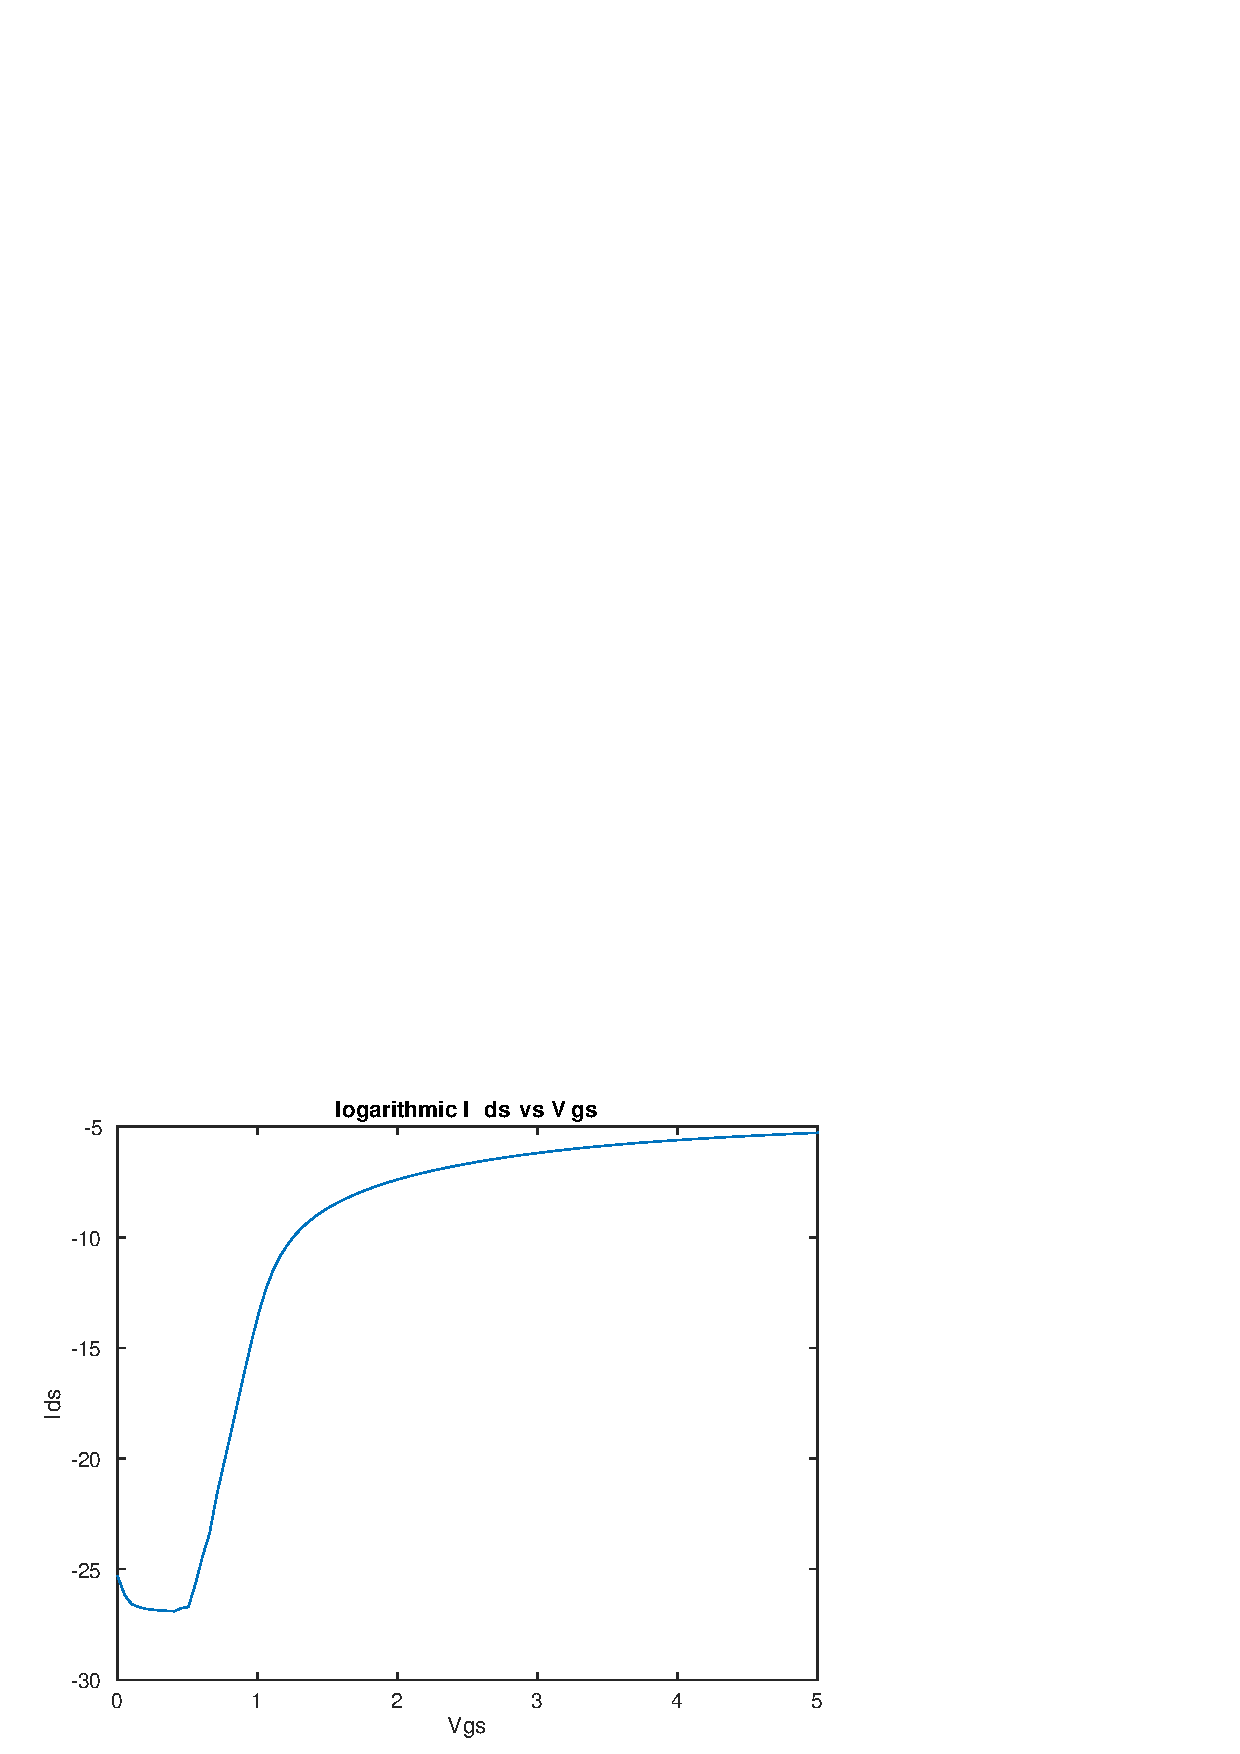
\includegraphics[scale=1]{task6log.png}
\end{figure}

\begin{figure}[ht!]
\caption{\textbf{task 8}}
\includegraphics[scale=0.9]{task8.png}
\end{figure}

\begin{figure}[ht!]
\caption{t\textbf{ask 9}}
\includegraphics[scale=1]{task9.png}
\end{figure}

\begin{figure}[ht!]
\caption{\textbf{task 10}}
\includegraphics[scale=1]{task10.png}
\end{figure}

\begin{figure}
\caption{\textbf{task 11}: $\sqrt{I_{ds}}$ vs $v_{gs}$}
\includegraphics[scale=1]{task11.jpg}
\end{figure}
\end{document}